\section{Experimental Methodology}
\label{sec:method}

This section describes how the counterfeit signal is generated, how it is checked
against a recorded attack, how the library of transmitter settings is built, what the
fourteen detectors are, and how they are set to a common operating point.

\subsection{Corpus and receiver configuration}
\label{sec:corpus}

The authentic signal is the cleanStatic recording of the Texas Spoofing Test Battery
\citep{humphreys2012texbat}. It holds raw in-phase and quadrature samples of the GPS L1
band taken at a surveyed stationary antenna, at 25 million complex samples per second
with 16 bits in each component. It contains no spoofing, so it supplies an authentic
signal that a counterfeit can be added to.

All tracking is performed by FGI-GSRx \citep{fgigsrx}, an open software receiver. Using
a published receiver matters for two reasons. The measurements the detectors read are
the ones a real integrity monitor would compute, and any reader can reproduce them from
the same recordings with the same software.

\subsection{Spoofing waveform generation}
\label{sec:generator}

The counterfeit is built as radio samples and then added to the authentic samples.

The generator is seeded from the receiver's own tracking of the authentic recording. For
each satellite the receiver reports, at every millisecond, where it found the code, what
carrier frequency it is tracking and how strong the signal is. Those quantities describe
the authentic signal as the receiver sees it, so they are exactly what a counterfeit
must match in order to arrive aligned. The generator reads them and produces, for each
satellite, a replica of the GPS L1 C/A signal at the same code phase, the same carrier
frequency and the same amplitude.

The attacker's settings of Table~\ref{tab:attacker} are then applied to that replica.
The power advantage scales its amplitude. The code offset and pull-off rate displace its
code, with the displacement growing at the chosen rate. The carrier offset and phase
shift its carrier.

The counterfeit and the authentic samples are summed, and the result passes through a
model of the receiver front end before being written. The front end applies automatic
gain control, which is the mechanism a real receiver uses to keep the signal inside the
range its converter can represent. When added power would drive the sum beyond that
range, the gain is reduced so that the sum still fits. This detail matters. Without it,
added power would clip, and the clipping would be an artefact of the file format instead
of a property of the attack.

The written file is then tracked by FGI-GSRx exactly as the authentic recording is, and
the measurements it produces are what the detectors read.

Two properties follow from building the attack this way. Every constraint a receiver
imposes is satisfied because a receiver produced the measurements, which covers the
continuity of code and carrier, the bandwidth and settling of the tracking loops, the
behaviour of the automatic gain control and the smoothness of the measurements from one
epoch to the next. No projection onto a set of allowed values is applied at any point,
because there is no perturbation to project.
Figure~\ref{fig:rxvalid} shows the checks on the receiver itself.

% Figure source: figures_src/fig_legacy.py
\begin{figure*}[t]
\centering
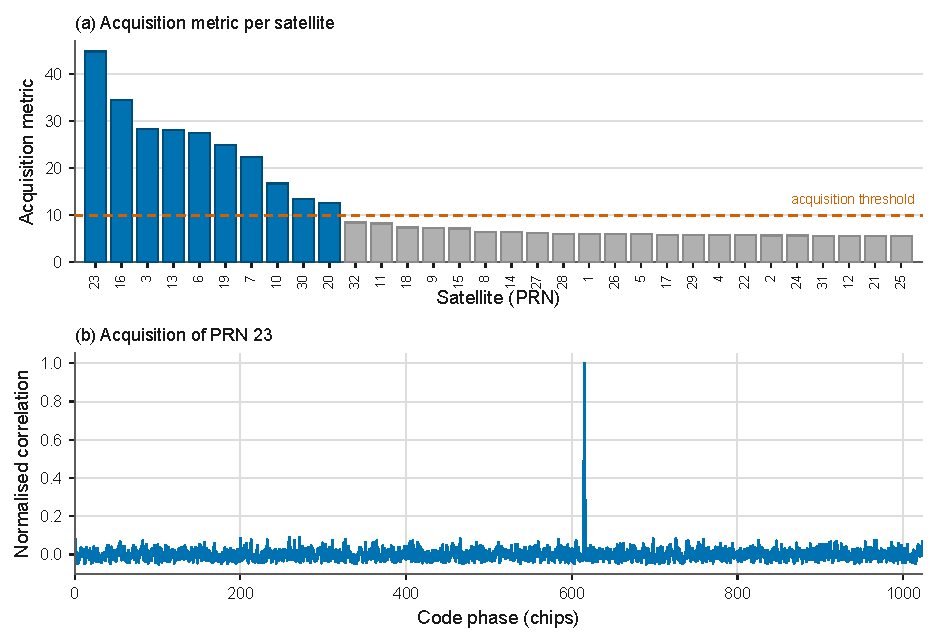
\includegraphics[width=\textwidth]{figures/fig04_receiver_validation.pdf}
\caption{Validation of the software receiver on the authentic recording. Panel (a) shows the acquisition metric for each satellite, and panel (b) shows the correlation against code phase for one satellite. Both match what a correctly operating receiver produces, which establishes that the measurements used throughout come from sound tracking.}
\label{fig:rxvalid}
\end{figure*}

\subsection{Generator validation}
\label{sec:validation}

A generator that cannot reproduce a documented attack is not evidence about attacks that
were never recorded. The check uses data set ds7 of the battery, whose construction is
published in full \citep{humphreys2016texbatds78}.

That document specifies ds7 as a power matched time push carried out with carrier phase
alignment. During the takeover the counterfeit phasor is
$P_s(t) = A_s(t)\,e^{j\theta(t)}$, with the angle $\theta$ rising from $\pi/2$ to $\pi$
and the amplitude following $A_s(t) = -2A_a\cos\theta(t)$, where $A_a$ is the authentic
amplitude. Those two choices together give a combined phasor
\begin{equation}
P_a + P_s = A_a + A_s e^{j\theta} = -A_a e^{j2\theta},
\label{eq:ds7takeover}
\end{equation}
whose magnitude stays at $A_a$ while its angle turns from $0$ to $\pi$. The victim's
loops are therefore walked onto the counterfeit with no step in power and no step in
phase. After the takeover the counterfeit holds at twice the authentic amplitude in
antipodal phase, so the sum returns to magnitude $A_a$, and the document records that
the victim's measurements match the clean recording apart from a carrier phase that is
greater by $\pi$. From then the code is dragged at 1.2 metres per second while the
counterfeit Doppler is held equal to the authentic Doppler.

Running the generator at those settings reproduces the recorded measurements.
Figure~\ref{fig:ds7} reports the comparison. Seven of the eight satellites agree within
half a decibel of carrier-to-noise density ratio. The eighth differs by more, and the
difference is not isolated: across the satellites the gap between generated and recorded
grows with the strength of the satellite, with a Spearman rank correlation of $+0.905$
at $p = 0.002$, and the trend remains when the strongest satellite is removed. The cause
is that the generated counterfeit is an amplitude matched replica, so the cancellation in
Equation~\ref{eq:ds7takeover} is cleaner than the recorded spoofer's hardware achieved,
which leaves the generated attack slightly louder. A slightly louder attack is easier to
detect, so this difference understates what an attacker can do.

\begin{figure*}[t]
\centering
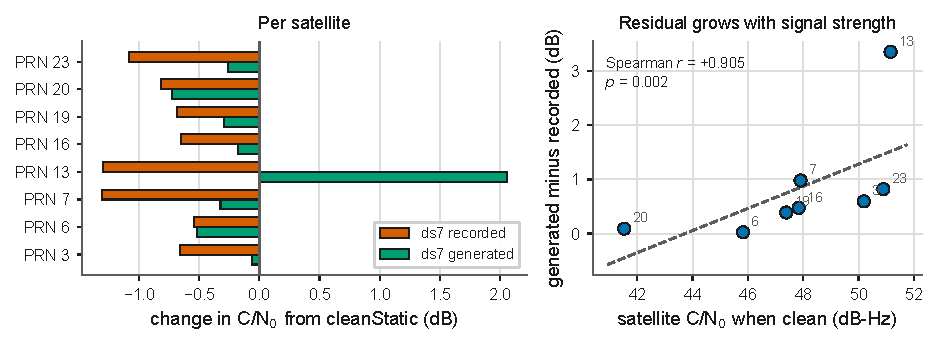
\includegraphics[width=\textwidth]{figures/fig_ds7_validation.pdf}
\caption{The generator reproduces the recorded ds7 attack. Left, the change in
carrier-to-noise density ratio from the clean recording, for the recorded attack and for
the generated one, per satellite. Right, the residual between them grows with satellite
strength, so the strongest satellite is the extreme of a trend and not an isolated
disagreement. The generated attack sits slightly above the recorded one, which makes it
easier to detect.}
\label{fig:ds7}
\end{figure*}

\subsection{Transmitted attack library}
\label{sec:library}

The attacker's choice set is expressed as a library. Each entry is one combination of
the settings in Table~\ref{tab:attacker}, and for each the generator produces a
composite file which the receiver tracks and the exporter turns into measurements. The
library holds 209 entries.

Two families of setting are covered. In the first the counterfeit carrier is in phase
with the authentic carrier, and the power advantage is swept from $-3$ to $10$ decibels.
The second follows the law of Equation~\ref{eq:ds7takeover}: for a counterfeit of
amplitude ratio $g$ at phase $\varphi$, the received power is unchanged when
\begin{equation}
g = -2\cos\varphi ,
\label{eq:neutral}
\end{equation}
so a counterfeit on this locus is invisible to a test that watches received power alone.
The ds7 attack sits on it at $\varphi = \pi$ and $g = 2$. Both families are crossed with
seven code pull-off rates from zero to 147 metres per second and three carrier alignment
settings.

Section~\ref{sec:threat} gives the two conditions a counterfeit must satisfy to take over
a receiver. Applied to the library, they select the entries where the counterfeit is
stronger than the authentic signal and is dragging the code. That is 126 of the 209
entries, and those 126 are the attacks the detectors are measured against.
Figure~\ref{fig:attackspace} shows the library and the subset.

\begin{figure}[t]
\centering
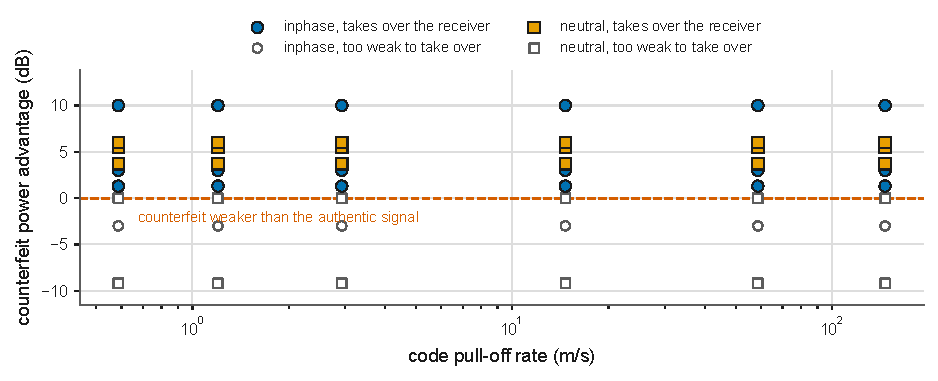
\includegraphics[width=\linewidth]{figures/fig_attack_space.pdf}
\caption{The transmitter settings in the library. Filled markers are the 126 settings
where the counterfeit is stronger than the authentic signal and is dragging the code,
which are the conditions for taking over a receiver. Open markers are settings that do
not meet them. Circles are the in phase family and squares follow the power neutral law
of Equation~\ref{eq:neutral}.}
\label{fig:attackspace}
\end{figure}

\subsection{Detector models and training}
\label{sec:detectors}

Fourteen detectors are tested. They are listed in Table~\ref{tab:detectors} with what
each one does, so that the comparison can be read without reference to the machine
learning literature. All fourteen read the same nine measurements described in
Section~\ref{sec:signal}.

\begin{table*}[t]
\centering
\caption{The fourteen detectors and the decision rule each one applies. The classical
models decide from the measurements of a single epoch. The deep networks decide from a
window of consecutive epochs, so they can use how the measurements change.}
\label{tab:detectors}
\begin{tabular}{@{}p{3.6cm}lp{7.0cm}@{}}
\toprule
Detector & Family & How it decides \\
\midrule
Decision tree      & classical & A sequence of threshold tests on single measurements,
                                 forming one branching rule \citep{breiman2001random} \\
Random forest      & classical & Many decision trees fitted to different samples of the
                                 data, whose votes are averaged \citep{breiman2001random} \\
Gradient boosting  & classical & Trees added one at a time, each fitted to the errors
                                 left by the previous ones \citep{friedman2001greedy} \\
XGBoost            & classical & Gradient boosting with additional penalties on tree
                                 complexity \citep{chen2016xgboost} \\
LightGBM           & classical & Gradient boosting that grows trees leaf by leaf for
                                 speed on large data \citep{ke2017lightgbm} \\
Nearest neighbour  & classical & Labels an epoch by the labels of the most similar
                                 training epochs \\
Support vector machine & classical & Places a boundary separating the classes with the
                                 widest margin, using a radial basis kernel \\
Multilayer perceptron & classical & A small feed forward network of fully connected
                                 layers \\
\midrule
One dimensional convolutional network & deep & Filters slid along the window respond to
                                 local patterns in time \\
Long short term memory & deep & Carries a state along the window, so earlier epochs
                                 inform later ones \citep{hochreiter1997long} \\
Bidirectional long short term memory & deep & The same, traversing the window in both
                                 directions \\
Convolutional recurrent hybrid & deep & Convolutional filters feeding a recurrent
                                 layer \\
Transformer        & deep & Weighs every epoch in the window against every other through
                                 attention \citep{vaswani2017attention} \\
Temporal convolutional network & deep & Dilated convolutions reaching across the window
                                 without recurrence \citep{bai2018empirical} \\
\bottomrule
\end{tabular}
\end{table*}

The set spans the families used in the detection literature reviewed in
Section~\ref{sec:rw_learning}, covering tree ensembles, instance based classification,
kernel methods, a feed forward network and the convolutional, recurrent, hybrid and
attention branches of sequence modelling.

\subsection{Feature space comparison}
\label{sec:comparison}

The attacks described above are transmitted. To show what a study that perturbed the
measurements instead would have concluded, each detector is also measured a second way,
and that measurement is reported alongside as a comparison.

The comparison uses a decision based boundary attack. It is given only the detector's
output decision for a sample, authentic or spoofed, and no gradient, no score and no
knowledge of the model. Starting from a spoofed sample the detector flags, and from an
authentic sample it does not, the attack performs a binary search along the line between
them to locate the point where the decision changes, then reduces the largest single
change across the nine measurements while keeping the decision on the authentic side.
The quantity reported is the smallest such change, measured in the normalised space where
each measurement is scaled to the unit interval, so the nine are comparable.

This is the appropriate comparison to make. A gradient attack would need access to the
detector's internals, and Section~\ref{sec:threat} states that the attacker in this study
has none. A decision based attack needs only the output decision, so it is the strongest
attack available to an adversary that cannot see inside the model
\citep{brendel2018decision,chen2020hopskipjump}. It is also the attack that a
non-differentiable detector cannot evade by denying gradients
\citep{athalye2018obfuscated}.

The comparison is reported for one purpose. It shows where a measurement space
evaluation and a transmitted attack agree about a detector and where they do not, which
Section~\ref{sec:res_compare} sets out. It is not used to support any claim about what a
spoofer can achieve, because a perturbation of the measurements is not by itself a signal
a transmitter can send.

\subsection{Operating point calibration}
\label{sec:oppoint}

A detector reports a score, and a threshold turns that score into a decision. Moving the
threshold trades two quantities against each other. Recall is the fraction of spoofed
samples that are flagged. The false alarm rate is the fraction of authentic samples that
are flagged. Raising the threshold lowers both, and lowering it raises both, so two
detectors read at different thresholds cannot be compared.

Every detector in this study is therefore set to one common operating point. The
threshold is the highest value at which the detector still flags 95 percent of the
spoofed samples in clean validation data,
\begin{equation}
\eta^\star = \max\{\eta : R_\mathrm{val}(\eta) \ge 0.95\},
\label{eq:oppoint}
\end{equation}
where $R_\mathrm{val}$ is recall on that data. A recall floor is the safety first choice
for an integrity monitor, because missing an attack is the failure that matters. The
false alarm rate each detector pays to meet that floor is reported alongside every
result, since a detector can always meet a recall floor by flagging everything.

The data are divided so that training, validation and test come from separate blocks of
each recording, with a gap discarded at every block boundary. Adjacent epochs of the same
satellite are nearly identical, because the tracking loops have time constants of order a
second, so a division that scattered neighbouring epochs across the blocks would place
near copies of the same measurement in training and in test and would inflate every
score.
